% Copyright (c) 2022 by Lars Spreng
% This work is licensed under the Creative Commons Attribution 4.0 International License. 
% To view a copy of this license, visit http://creativecommons.org/licenses/by/4.0/ or send a letter to Creative Commons, PO Box 1866, Mountain View, CA 94042, USA.

%~~~~~~~~~~~~~~~~~~~~~~~~~~~~~~~~~~~~~~~~~~~~~~~~~~~~~~~~~~~~~~~~~~~~~~~~~~~~~~
% You can add your packages and commands to the loadslides.tex file. 
% The files in the folder "styles" can be modified to change the layout and design of your slides.
% I have included examples on how to use the template below. 
% Some of it these examples are taken from the Metropolis template.
%~~~~~~~~~~~~~~~~~~~~~~~~~~~~~~~~~~~~~~~~~~~~~~~~~~~~~~~~~~~~~~~~~~~~~~~~~~~~~~


\documentclass[
11pt,notheorems,hyperref={pdfauthor=whatever}
]{beamer}


% Copyright (c) 2022 by Lars Spreng
% This work is licensed under the Creative Commons Attribution 4.0 International License. 
% To view a copy of this license, visit http://creativecommons.org/licenses/by/4.0/ or send a letter to Creative Commons, PO Box 1866, Mountain View, CA 94042, USA.

%~~~~~~~~~~~~~~~~~~~~~~~~~~~~~~~~~~~~~~~~~~~~~~~~~~~~~~~~~~~~~~~~~~~~~~~~~~~~~~
% Add your packages and commands to this file
%~~~~~~~~~~~~~~~~~~~~~~~~~~~~~~~~~~~~~~~~~~~~~~~~~~~~~~~~~~~~~~~~~~~~~~~~~~~~~~



%~~~~~~~~~~~~~~~~~~~~~~~~~~~~~~~~~~~~~~~~~~~~~~~~~~~~~~~~~~~~~~~~~~~~~~~~~~~~~~
\RequirePackage{palatino}
\RequirePackage[utf8]{inputenc}
\RequirePackage[T1]{fontenc}
\RequirePackage{}
\usepackage{intcalc}
\usefonttheme{serif}

\usepackage{styles/elegantmacros}
\usefolder{styles}
\usetheme[style=blue]{elegant}



\newcommand{\makepart}[1]{ % For convenience
\part{#1} \frame{\partpage}
}

%~~~~~~~~~~~~~~~~~~~~~~~~~~~~~~~~~~~~~~~~~~~~~~~~~~~~~~~~~~~~~~~~~~~~~~~~~~~~~~

%~~~~~~~~~~~~~~~~~~~~~~~~~~~~~~~~~~~~~~~~~~~~~~~~~~~~~~~~~~~~~~~~~~~~~~~~~~~~~~
% Figures
\RequirePackage{booktabs}
\RequirePackage{colortbl}
\RequirePackage{ragged2e}
\RequirePackage{schemabloc}
%\RequirePackage{natbib}
\RequirePackage{caption}
\RequirePackage{subcaption}
\RequirePackage{tabularx}
\RequirePackage{colortbl}
\RequirePackage{array}
\RequirePackage{multirow}
\usepackage[
  style=authoryear, 
]{biblatex}
\addbibresource{references.bib}
\newcolumntype{Y}{>{\centering\arraybackslash}X}

%~~~~~~~~~~~~~~~~~~~~~~~~~~~~~~~~~~~~~~~~~~~~~~~~~~~~~~~~~~~~~~~~~~~~~~~~~~~~~~

%~~~~~~~~~~~~~~~~~~~~~~~~~~~~~~~~~~~~~~~~~~~~~~~~~~~~~~~~~~~~~~~~~~~~~~~~~~~~~~
% Figures
\RequirePackage{wrapfig}
\usepackage{pgfplots}
\pgfplotsset{compat=1.18}
\RequirePackage{graphicx}
\RequirePackage{adjustbox}
\RequirePackage{environ}
%\pgfplotsset{compat=1.18}


\makeatletter
\RequirePackage{tikz}
\usepgfplotslibrary{fillbetween}
\usetikzlibrary{patterns, shapes.geometric}
    
\newsavebox{\measure@tikzpicture}
\NewEnviron{scaletikzpicturetowidth}[1]{%
  \def\tikz@width{#1}%
  \def\tikzscale{1}\begin{lrbox}{\measure@tikzpicture}%
  \BODY
  \end{lrbox}%
  \pgfmathparse{#1/\wd\measure@tikzpicture}%
  \edef\tikzscale{\pgfmathresult}%
  \BODY
}
\usetikzlibrary{ducks}
\makeatother
%~~~~~~~~~~~~~~~~~~~~~~~~~~~~~~~~~~~~~~~~~~~~~~~~~~~~~~~~~~~~~~~~~~~~~~~~~~~~~~

%~~~~~~~~~~~~~~~~~~~~~~~~~~~~~~~~~~~~~~~~~~~~~~~~~~~~~~~~~~~~~~~~~~~~~~~~~~~~~~
% Colors

\definecolor{sangue}{HTML}{780000}
\definecolor{sanguechiaro}{HTML}{C1121F}
\definecolor{muro}{HTML}{FDF0D5}
\definecolor{sera}{HTML}{003049}
\definecolor{macchina}{HTML}{669BBC}

%~~~~~~~~~~~~~~~~~~~~~~~~~~~~~~~~~~~~~~~~~~~~~~~~~~~~~~~~~~~~~~~~~~~~~~~~~~~~~~
%My fun

\newcommand{\myemph}[1]{\textcolor{sera}{#1}}

 %~~~~~~~~~~~~~~~~~~~~~~~~~~~~~~~~~~~~~~~~~~~~~~~~~~~~~~~~~~~~~~~~~~~~~~~~~~~~~~

%~~~~~~~~~~~~~~~~~~~~~~~~~~~~~~~~~~~~~~~~~~~~~~~~~~~~~~~~~~~~~~~~~~~~~~~~~~~~~~
% Maths 
\RequirePackage{textcomp}
\RequirePackage{amsmath} 
\RequirePackage{amsthm}
\RequirePackage{mathtools}
\usepackage{amsfonts}
\usepackage{amssymb}
\usepackage{eurosym}
\usepackage{float}
\usepackage{xfrac}
\usepackage{mathrsfs} 

%\RequirePackage{bbm}
%\RequirePackage{algorithm}
%\RequirePackage[osf,sc]{mathpazo}
%\RequirePackage{pifont}
%\newcommand{\xmark}{\ding{55}}%
%\numberwithin{equation}{section}
\DeclareMathOperator*{\argmax}{arg\,max}
\DeclareMathOperator*{\argmin}{arg\,min}

%define theorems
% \newtheorem{assumption}{Assumption}
% \newtheorem{theorem}{Theorem}
\newtheorem{prop}{Proposition}
\newtheorem{observation}{Observation}

% Define mathematical symbols
\newcommand{\nc}{\newcommand}
\nc{\sS}{ \mathscr{S}}
\nc{\sC}{ \mathscr{C}}
\nc{\cH}{{\mathcal H}}
\nc{\cR}{{\mathcal R}}
\nc{\cA}{{\mathcal A}}
\nc{\cG}{{\mathcal G}}
\nc{\cC}{{\mathcal C}}
\nc{\cD}{{\mathcal D}}
\nc{\cO}{{\mathcal O}}
\nc{\cI}{{\mathcal I}}
\nc{\cB}{{\mathcal B}}
\nc{\cY}{{\mathcal Y}}
\nc{\cK}{{\mathcal K}} 
\nc{\cX}{{\mathcal X}}
\nc{\cS}{{\mathcal S}}
\nc{\cE}{{\mathcal E}}
\nc{\cF}{{\mathcal F}}
\nc{\cZ}{{\mathcal Z}}
\nc{\cQ}{{\mathcal Q}}
\nc{\cP}{{\mathcal P}}
\nc{\cL}{{\mathcal L}}
\nc{\cM}{{\mathcal M}}
\nc{\cN}{{\mathcal N}}
\nc{\cT}{{\mathcal T}}
\nc{\cW}{{\mathcal W}}
\nc{\cU}{{\mathcal U}}
\nc{\cJ}{{\mathcal J}}
\nc{\cV}{{\mathcal V}}
\nc{\bH}{{\mathbb H}}
\nc{\bA}{{\mathbb A}}
\nc{\bG}{{\mathbb G}}
\nc{\bC}{{\mathbb C}}
\nc{\bO}{{\mathbb O}}
\nc{\bI}{{\mathbb I}}
\nc{\bB}{{\mathbb B}}
\nc{\bY}{{\mathbb Y}}
\nc{\bK}{{\mathbb K}} 
\nc{\bX}{{\mathbb X}}
\nc{\bS}{{\mathbb S}}
\nc{\bE}{{\mathbb E}}
\nc{\bF}{{\mathbb F}}
\nc{\bZ}{{\mathbb Z}}
\nc{\bQ}{{\mathbb Q}}
\nc{\bN}{{\mathbb N}}
\nc{\bP}{{\mathbb P}}
\nc{\bL}{{\mathbb L}}
\nc{\bM}{{\mathbb M}}
\nc{\bT}{{\mathbb T}}
\nc{\bW}{{\mathbb W}}
\nc{\bU}{{\mathbb U}}
\nc{\bD}{{\mathbb D}}
\nc{\bJ}{{\mathbb J}}
\nc{\bV}{{\mathbb V}}
\nc{\bR}{{\mathbb R}}

% & \frac{1}{J} \sum_{s \in \cJ} \sum_{t \in \cT} \Bigg(\sum_{i \in \netN}
% \left( c_i^\aHtE \HtEi + c_i^\aEtH \EtHi \right) + \\
%  & \hspace{2cm} \sum_{l \in \netE_H} \cHedge |\Hedgej| + \sum_{l\in \netE_P} \cPedge |\Pedgej| \Bigg),
%MOPTA PACKAGES AND COMMANDS

\nc{\boB}{{\mathbf{B}}}
\nc{\boL}{{\mathbf{L}}}
\nc{\boY}{{\mathbf{Y}}}
\nc{\boI}{{\mathbf{I}}}
\nc{\boV}{{\mathbf{V}}}
\nc{\boS}{{\mathbf{S}}}
\nc{\tV}{{\Tilde{{V}}}}
\nc{\tI}{{\Tilde{{I}}}}
\nc{\tY}{{\Tilde{{Y}}}}
\nc{\tS}{{\Tilde{{S}}}}
\nc{\fr}{{\rightarrow}}
\nc{\co}{{\nabla}}
\nc{\E}{\mathbb{E}}
\nc{\CG}{C_{\Sigma}^{\text{Gauss}}}



\newcommand{\virgolette}[1]{``#1''} %\virgolette{questo č fra virgolette}%
%\usepackage{frontespizio}
\newcommand{\abs}[1]{\lvert#1\rvert}


\DeclareMathOperator{\diag}{diag}
\DeclareMathOperator{\dw}{d_w}
\DeclareMathOperator{\C}{C_{tc}}
\DeclareMathOperator{\T}{T}
\DeclareMathOperator{\MP}{MP}
\DeclareMathOperator{\KP}{KP}
\DeclareMathOperator{\K}{K}
\DeclareMathOperator{\Id}{Id}
\DeclareMathOperator{\SSpan}{Span}
\DeclareMathOperator{\epi}{epi}
\DeclareMathOperator{\supp}{supp}

%%comandi per LP
\nc{\cost}{c}
\nc{\Av}{A}
\nc{\xv}{x}
\nc{\bv}{b}
\nc{\rhov}{\rho}
\nc{\At}{\tilde{A}}
\nc{\xt}{\tilde{x}}
\nc{\bt}{\tilde{b}}
\nc{\var}{Var}
\nc{\row}{R}
\nc{\col}{C}
\nc{\rowP}{\sigma}
\nc{\colP}{\delta}
\nc{\rowW}{\omega}
\nc{\colW}{\tau}


%% comandi per le variabili:
\nc{\Tmax}{\text{$T_{\text{max}}$}}
\nc{\xvar}{\textcolor{sanguechiaro}{\text{$x$}}}
\nc{\nsi}{\textcolor{sangue}{\text{$x_i^{(p)}$}}}
\nc{\nwi}{\textcolor{sangue}{\text{$x_i^{(w)}$}}}
\nc{\nhi}{\textcolor{sangue}{\text{$x_i^{(h)}$}}}
\nc{\mhtei}{\textcolor{sangue}{\text{$x_i^{(h\rightarrow e)}$}}}
\nc{\methi}{\textcolor{sangue}{\text{$x_i^{(e\rightarrow h)}$}}}

\nc{\nsit}{\textcolor{sangue}{\text{$\tilde{x}_i^{(p)}$}}}
\nc{\nwit}{\textcolor{sangue}{\text{$\tilde{x}_i^{(w)}$}}}
\nc{\nhit}{\textcolor{sangue}{\text{$\tilde{x}_i^{(h)}$}}}

\nc{\ns}{\textcolor{sangue}{\text{$x^{(p)}$}}}
\nc{\nw}{\textcolor{sangue}{\text{$x^{(w)}$}}}
\nc{\nh}{\textcolor{sangue}{\text{$x^{(h)}$}}}
\nc{\mhte}{\textcolor{sangue}{\text{$x^{(h\rightarrow e)}$}}}
\nc{\meth}{\textcolor{sangue}{\text{$x^{(e\rightarrow h)}$}}}

\nc{\addNTC}{\textcolor{sangue}{\text{$y^{(e)}$}}}
\nc{\addMH}{\textcolor{sangue}{\text{$y^{(h)}$}}}
\nc{\addNTCj}{\textcolor{sangue}{\text{$y_l^{(e)}$}}}
\nc{\addMHj}{\textcolor{sangue}{\text{$y_l^{(h)}$}}}
\nc{\aHtE}{\text{${(h \rightarrow e)}$}}
\nc{\aEtH}{\text{${(e \rightarrow h)}$}}

\nc{\zvar}{\textcolor{macchina}{\text{$z$}}}
\nc{\Zvar}{\text{$\textcolor{sera}{\cZ(}\xvar\textcolor{sera}{)}$}}
\nc{\Pedge}{\textcolor{macchina}{\text{$z^{(e)}$}}}
\nc{\Hedge}{\textcolor{macchina}{\text{$z^{(h)}$}}}
\nc{\Pedgej}{\textcolor{macchina}{\text{$z_{l\omega t}^{(e)}$}}}
\nc{\Hedgej}{\textcolor{macchina}{\text{$z_{l\omega t}^{(h)}$}}}
\nc{\Pedgejj}[3]{\textcolor{macchina}{\text{$z_{#1 #2 #3}^{(e)}$}}}
\nc{\Hedgejj}[3]{\textcolor{macchina}{\text{$z_{#1 #2 #3}^{(h)}$}}}

\nc{\HtEi}{\textcolor{macchina}{\text{$z_{i\omega t}^{(h \rightarrow e)}$}}}
\nc{\EtHi}{\textcolor{macchina}{\text{$z_{i\omega t}^{(e \rightarrow h)}$}}}
\nc{\HtEii}[3]{\textcolor{macchina}{\text{$z_{#1 #2 #3}^{(h \rightarrow e)}$}}}
\nc{\EtHii}[3]{\textcolor{macchina}{\text{$z_{#1 #2 #3}^{(e \rightarrow h)}$}}}
\nc{\tildeHtE}[3]{\textcolor{macchina}{\text{$\tilde{z}_{#1 #2 #3}^{(h \rightarrow e)}$}}}
\nc{\tildeEtH}[3]{\textcolor{macchina}{\text{$\tilde{z}_{#1 #2 #3}^{(e \rightarrow h)}$}}}

\nc{\HS}{\textcolor{macchina}{\text{$z$}}}
\nc{\dHS}{\textcolor{macchina}{\text{$z^{\Delta}$}}}
\nc{\HSj}{\textcolor{macchina}{\text{$z_{ist}$}}}
\nc{\dHSj}{\textcolor{macchina}{\text{$z_{ist}^{\Delta}$}}}
\nc{\HSjj}[3]{\textcolor{macchina}{\text{$z_{#1 #2 #3}$}}}
\nc{\tildeHS}[3]{\textcolor{macchina}{\text{$\tilde{z}_{#1 #2 #3}$}}}
\nc{\dHSjj}[3]{\textcolor{macchina}{\text{$z_{#1 #2 #3}^{\Delta}$}}}
\nc{\tildedHS}[3]{\textcolor{macchina}{\text{$\tilde{z}_{#1 #2 #3}^{\Delta}$}}}

\nc{\rHbalance}{r^{\text{H}}}
\nc{\rPbalance}{r^{\text{P}}} 


%% comandi per i parametri 

\nc{\aggcost}{\tilde{\cost}}
\nc{\chte}{c_i^{(h \rightarrow e)}}
\nc{\ceth}{c_i^{(e \rightarrow h)}}
\nc{\cHedge}{c_l^{(h)}}
\nc{\cPedge}{c_l^{(e)}}
\nc{\cNTC}{d_l^{(e)}}
\nc{\cMH}{d_l^{(h)}}
\nc{\cmhte}{b_i^{(e \rightarrow h)}}
\nc{\cmeth}{b_i^{(h \rightarrow e)}}

\nc{\fhte}{f_i^\aHtE}
\nc{\feth}{f_i^\aEtH}
\nc{\NTC}{a_l^{(e)}}
\nc{\MH}{a_l^{(h)}}

\nc{\Mns}{\text{$Mns$}}
\nc{\Mnw}{\text{$Mnw$}}
\nc{\Mnh}{\text{$Mnh$}}
\nc{\Mhte}{\text{$Mhte$}}
\nc{\Meth}{\text{$Meth$}}

\nc{\ES}{\text{$E_{i\omegat}^{(e)}$}}
\nc{\EW}{\text{$W_{i\omegat}^{(e)}$}}
\nc{\EL}{\text{$L_{i\omegat}^{(e)}$}}
\nc{\HL}{\text{$L_{i\omegat}^{(h)}$}}
\nc{\ESt}[1]{\text{$E_{i\omega#1}^{(e)}$}}
\nc{\EWt}[1]{\text{$W_{i\omega#1}^{(e)}$}}
\nc{\ELt}[1]{\text{$L_{i\omega#1}^{(e)}$}}
\nc{\HLt}[1]{\text{$L_{i\omega#1}^{(h)}$}}
\nc{\slack}{s}
%% commandi per i grafi
\nc{\netN}{\cN}
\nc{\netE}{\cL}
\nc{\aggN}{\cN}
\nc{\aggE}{\cE}
\nc{\adje}{\delta}
\nc{\outn}{\adje^+}
\nc{\inn}{\adje^-}
%% unità di misura
\nc{\power}{\text{MWh}}


%% comandi per timepartition
\nc{\timeP}{\cP}
\nc{\CEP}{CEP}
\nc{\CEPT}{\CEP\(_{\cT}\;\)}
\nc{\CEPP}{\CEP\(_{\timeP}\)}
\nc{\mCEPT}{\text{\CEP}_{\cT}}
\nc{\mCEPP}{\text{\CEP}_{\timeP}}
\nc{\prob}{P}

\newcommand{\duckone}{
  \duck[beret=red!70!black,
        signpost=\scalebox{0.4}{
          \parbox{2cm}{\color{black}
          \centering Intraday\\ Duck}},
        signcolour=brown!70!gray,
        signback=white!80!brown]
  }

  \newcommand{\ducktwo}{
    \duck[witch=black!50!gray,
          jacket=black!50!gray,
          signpost=\scalebox{0.4}{
            \parbox{2cm}{\color{black}
            \centering Annual \\ Duck}},
          signcolour=brown!70!gray,
          signback=white!80!brown]
    }


\setbeamertemplate{theorems}[numbered] % to number

\theoremstyle{definition}
\newtheorem{fact}{Fact}[section]
\newtheorem{examp}{Example}[section]

\theoremstyle{plain}
\newtheorem{definition}{Definition}[section]
\newtheorem{proposition}{Proposition}
\newtheorem{theorem}{Theorem}
\newtheorem{assumption}{Assumption}

%%cell command
\newcommand{\cell}[2]{%
    \begin{tabular}{|c|}
     \hline \cellcolor{#2} #1 \\ \hline
    \end{tabular}
}

\providecommand{\H}{\mathscr{H}}      
\providecommand{\E}{\mathbb{E}}
\makeatletter
\def\munderbar#1{\underline{\sbox\tw@{$#1$}\dp\tw@\z@\box\tw@}}
\makeatother

%~~~~~~~~~~~~~~~~~~~~~~~~~~~~~~~~~~~~~~~~~~~~~~~~~~~~~~~~~~~~~~~~~~~~~~~~~~~~~~

%\usepackage{xcolor}

 % Loads packages and some defined commands

\title[\hspace{-3.0cm} Projective Metrics %\hspace{2.5cm}  JWCC 2023
% Text entered here will appear in the bottom middle
]{Projective Metrics}

%\subtitle{Presentation Subtitle}

\author[
Gabor Riccardi
% Text entered here will appear in the bottom left corner
]{
     Gabor Riccardi
}

\institute{
    University of Pavia (UniPv) \\\text{} \\ with \textbf{Hugo Sauerbier Couvée
}, Technical University of Munich (TUM)}
\date{20 September 2023}


\usepackage[outline]{contour}


\begin{document}

\theoremstyle{definition}
\newtheorem*{fact*}{Fact}
\newtheorem*{examp*}{Example}

\theoremstyle{plain}
\newtheorem*{definition*}{Definition}
\newtheorem*{proposition*}{Proposition}
\newtheorem*{theorem*}{Theorem}
\newtheorem*{assumption*}{Assumption}

\newcommand{\A}{\mathcal{A}}
\newcommand{\B}{\mathcal{B}}
%\newcommand{\C}{\mathcal{C}}


% Generate title page
{
\setbeamertemplate{footline}{} 
\begin{frame}
  \titlepage
\end{frame}
}
\addtocounter{framenumber}{-1}

% You can declare different parts as a parentof sections
%\begin{frame}{Part I: Demo Presentation Part}
%    \tableofcontents[part=1]
%\end{frame}
%\begin{frame}{Part II: Demo Presentation Part 2}
%    \tableofcontents[part=2]
%\end{frame}

%\setcounter{part}{-1}
%\makepart{Motivation}

\begin{frame}{Introduction to Coding Theory}

    \begin{itemize}
        \item Retrieve information from corrupted messages \pause
        \item Store data (which is just sending a message to your future self) \pause
        \item Data compression \pause
        \item Cryptography 
    \end{itemize}
\end{frame}
\begin{frame}

    \vspace{-2cm} % Adjust the vertical space as needed
    \hspace{2.3cm}\textcolor{red}{How?} \pause 
    \begin{center}
        \alert<1>{\Huge Redundancy!} \\ \pause
        \alert<3>{\huge (Smartly)}
    \end{center}
    \pause
    Let's repeat each row of a message three times and then send it.\\ \pause
    If we obtain the message:
    \pause
    \only<5>{
    \begin{center}
         \begin{tabular}{|c|c|c|c|c|c|c|c|c|}
        \hline
        0 & 0 & 0 & 1 & 0 & 1 & 0 & 0 & 0 \\
        \hline
        0 & 0 & 0 & 1 & 1 & 1 & 0 & 0 & 0 \\
        \hline
        0 & 0 & 0 & 1 & 1 & 1 & 0 & 0 & 0 \\
        \hline
        \end{tabular}
    \end{center}
    }
    
    \uncover<6->{
    \begin{center}
         \begin{tabular}{|c|c|c|c|c|c|c|c|c|}
        \hline
        0 & 0 & 0 & 1 & \cellcolor{red!20}0 & 1 & 0 & 0 & 0 \\
        \hline
        0 & 0 & 0 & 1 & \cellcolor{red!20} 1 & 1 & 0 & 0 & 0 \\
        \hline
        0 & 0 & 0 & 1 & \cellcolor{red!20} 1 & 1 & 0 & 0 & 0 \\
        \hline
        \end{tabular}
            
    \end{center}
    }
    \pause
    \bigskip
    
    Since "1" appears twice and "0" once, we may assume more likely that the original message was:
    \pause
    \bigskip
    
    \begin{center}
    \begin{tabular}{|c|c|c|c|c|c|c|c|c|}
        \hline
        0 & 0 & 0 & 1 & \cellcolor{green!20} 1 & 1 & 0 & 0 & 0 \\
        \hline
    \end{tabular}
    \end{center}
    \pause
    \bigskip
    
    But this way, we took three times the length of the message to correct one error!
    
    \bigskip
    \pause
    \textcolor{gray}{Btw the message says SOS in Morse, so maybe go seek help.}
    \end{frame}
    
\begin{frame}{A better way to do it}
We rearrange the original message
\begin{tabular}{|c|c|c|c|c|c|c|c|c|}
    \hline
    \rowcolor{blue!20} 0 & 0 & 0 & 1 &  1 & 1 & 0 & 0 & 0 \\
    \hline
\end{tabular}
in a 4 by 4 grid: \\ 
\begin{center}
\pause
\begin{tabular}{|c|c|c|c|}
\hline
     &  \cellcolor{red!20} 0 & \cellcolor{red!20} 0 & \cellcolor{blue!20}  0  \\ \hline
    \cellcolor{red!20} 1 & \cellcolor{blue!20} 0 & \cellcolor{blue!20}  0 & \cellcolor{blue!20} 1  \\ \hline
    \cellcolor{red!20} 0 & \cellcolor{blue!20} 1 &\cellcolor{blue!20}  1 &\cellcolor{blue!20} 0  \\ \hline
    \rowcolor{blue!20}0 & 0 & 0 & 0  \\ \hline
\end{tabular}
\end{center}
\pause
Where the red cells are the four redundant bits which encode the parity of subsets of columns or rows in the following way. \\
\pause
\only<4>{   
\begin{minipage}{0.4\textwidth}
        \begin{center}
    \begin{tabular}{|c|c|c|c|}
        \hline
          &  \cellcolor{red!35} 0 & 0 & \cellcolor{blue!20}  0  \\ \hline
        1 & \cellcolor{blue!20} 0 &  0 & \cellcolor{blue!40} 1  \\ \hline
        0 & \cellcolor{blue!40} 1 &  1 &\cellcolor{blue!20} 0  \\ \hline
        0 & \cellcolor{blue!20} 0 & 0 &  \cellcolor{blue!20} 0  \\ \hline
\end{tabular}
\end{center}
\end{minipage}
%
\begin{minipage}{0.4 \textwidth}
    \begin{center}
        \cell{0}{red!35} = \cell{1}{blue!40} + \cell{1}{blue!40}
    \end{center}
\end{minipage}
}
\only<5>{   
\begin{minipage}{0.4\textwidth}
        \begin{center}
    \begin{tabular}{|c|c|>{\columncolor{blue!20}}c|>{\columncolor{blue!20}}c|c|} 
    \hline
          &  0 & \cellcolor{red!30}0  &  0  \\ \hline
        1 & 0 &  0 & \cellcolor{blue!40}1  \\ \hline
        0 & 1 &  \cellcolor{blue!40}1 & 0  \\ \hline
        0 & 0 & 0 &  0  \\ \hline
\end{tabular}
\end{center}
\end{minipage}
%
\begin{minipage}{0.4 \textwidth}
    \begin{center}
        \cell{0}{red!35} = \cell{1}{blue!40} + \cell{1}{blue!40}
    \end{center}
\end{minipage}
}
\only<6>{   
\begin{minipage}{0.4\textwidth}
        \begin{center}
    \begin{tabular}{|c|c|c|c|}
        \hline
          &  0 & 0 &  0  \\ \hline
        \rowcolor{blue!20} \cellcolor{red!30}1 & 0 &  0 & \cellcolor{blue!40}1  \\ \hline
        0 & 1 &  1 & 0  \\ \hline
        \rowcolor{blue!20} 0 & 0 & 0 &  0  \\ \hline
\end{tabular}
\end{center}
\end{minipage}
%
\begin{minipage}{0.4 \textwidth}
    \begin{center}
        \cell{1}{red!35} = \cell{1}{blue!40} 
    \end{center}
\end{minipage}
}
\uncover<7->{
\begin{minipage}{0.4\textwidth}
        \begin{center}
    \begin{tabular}{|c|c|c|c|}
        \hline
          &  0 & 0 &  0  \\ \hline
        1 & 0 &  0 & 1  \\ \hline
        \rowcolor{blue!20} \cellcolor{red!35}0 & \cellcolor{blue!40} 1 &  \cellcolor{blue!40} 1 & 0  \\ \hline
        \rowcolor{blue!20} 0 & 0 & 0 &  0  \\ \hline
\end{tabular}
\end{center}
\end{minipage}
%
\begin{minipage}{0.4 \textwidth}
    \begin{center}
        \cell{0}{red!35} = \cell{1}{blue!40} + \cell{1}{blue!40}
    \end{center}
\end{minipage}
}
\hfill \\
\bigskip
\pause
\uncover<8->{
Since \(2^4 = \text{total number of bits} + (\text{case in which there is no error}) = 15 + 1\) and if there is up to one error, every redundant bit halvens the number the possible locations of where the error might be, we can always correct up to one error in the message.}
\end{frame}
\begin{frame}{Hamming Codes}
    
    The subset of codes in $\bF_2^{15}$ constructed the same way are called \textbf{Hamming Codes}.  \pause \\
    \vspace{0.5cm}
    \begin{minipage}{0.25\textwidth}
        \centering
        \begin{tabular}{|c|c|c|c|}
            \hline
            &  \cellcolor{red!20} 0 & \cellcolor{red!20} 0 & \cellcolor{blue!20}  1 \\ \hline
            \cellcolor{red!20} 0 & \cellcolor{blue!20} 0 & \cellcolor{blue!20}  0 & \cellcolor{blue!20} 1  \\ \hline
            \cellcolor{red!20} 1 & \cellcolor{blue!20} 0 &\cellcolor{blue!20}  1 &\cellcolor{blue!20} 1  \\ \hline
             \rowcolor{blue!20}0 & 1 & 0 & 0  \\ \hline
        \end{tabular}
    \end{minipage}
    %
    \begin{minipage}{0.05\textwidth}
    \centering
        \textbf{+}
    \end{minipage}
    %
    \begin{minipage}{0.25\textwidth}
    \centering
        \begin{tabular}{|c|c|c|c|}
            \hline
            &  \cellcolor{red!20} 0 & \cellcolor{red!20} 0 & \cellcolor{blue!20}  0 \\ \hline
            \cellcolor{red!20} 1 & \cellcolor{blue!20} 0 & \cellcolor{blue!20}  0 & \cellcolor{blue!20} 1  \\ \hline
            \cellcolor{red!20} 0 & \cellcolor{blue!20} 1 &\cellcolor{blue!20}  1 &\cellcolor{blue!20} 0  \\ \hline
             \rowcolor{blue!20}0 & 0 & 0 & 0  \\ \hline
        \end{tabular}
    \end{minipage}
    %
    \begin{minipage}{0.05\textwidth}
    \centering
        \textbf{=}
    \end{minipage}
%
    \begin{minipage}{0.25\textwidth}
    \centering
        \begin{tabular}{|c|c|c|c|}
            \hline
            &  \cellcolor{red!20} 0 & \cellcolor{red!20} 0 & \cellcolor{blue!20}  1 \\ \hline
            \cellcolor{red!20} 1 & \cellcolor{blue!20} 0 & \cellcolor{blue!20}  0 & \cellcolor{blue!20} 0  \\ \hline
            \cellcolor{red!20} 1 & \cellcolor{blue!20} 1 &\cellcolor{blue!20}  0 &\cellcolor{blue!20} 1  \\ \hline
             \rowcolor{blue!20}0 & 1 & 0 & 0  \\ \hline
        \end{tabular}
    \end{minipage} \\
\bigskip \pause
We observe that if we sum two Hamming codes, it remains an Hamming code (that is the parity checks remain valid also for the result of the sum): \\
\pause
     Thus, since we can choose the numbers inside the 11 blue cells arbitrarily they form a 11 dimensional linear subspace of $\bF_2^{15}$.  For this reason these codes are referred to as \textcolor{blue}{[15,11] Hamming Codes}.
     
\end{frame}

\begin{frame}{What are we actually doing when decoding a message?}
\begin{itemize}
    \item Note given a code in \(\bF^{15}_2\) by changing one bit we can always recover an Hamming Code. Thus what we are doing to correct a message is simply taking the closest valid message! 
    \pause
    \item We partition the message space into balls centered on the codewords. If we receive a message, then we simply look at what ball it is in and then the center of that ball is the most likely correct message (This is called \textcolor{blue}{nearest neighbour decoder (nnd)}).
    \pause
    \item To decode as many messages as possible, we take the largest radius such that the balls remain disjoint. 
    \pause
    \item This radius equals to \( \lfloor \frac{d-1}{2}\rfloor\) where \(d\) is \emph{the minimum distance} of the code (the set containing all the \(m\) codewords).
    \pause
    \item The minimum distance \(d\) is a simple measure of the goodness of a code.
    %\item (If the bit errors are i.i.d. then the nnd equals the maximum likelyhood decoder.)
    
    
   

    %if we center around each codeword in the alphabet a ball of size r and the balls are disjoint then r represents the number of errors we can correct in a code! We want the biggest r given the size of an alphabet-----) Sphere Packing
    
\end{itemize}

\end{frame}

\begin{frame}{Classical Sphere Packing Results}
\begin{itemize}
    \item Given a message length \(n\) and a minimum distance \(d\), we want to find the largest code with minimum distance \(d\). \\
    \item This can also be seen as the sphere packing problem for spheres of radius \(\lfloor \frac{d-1}{2}\rfloor\). 
\end{itemize}
\quad

\begin{theorem}[Hamming Bound] \label{hamming}
    Let \(\cC < \bF_q^n \) be a code with \(d_H(\cC) = d\) then:
\[|\cC|\leq \frac{q^n}{\sum_{i=o}^t\binom{n}{i}(q-1)^i}\] \\

Where \(t \coloneqq \lfloor \frac{d-1}{2}\rfloor \).
\end{theorem}

\begin{theorem}[Singleton Bound] \label{singleton}
Let \(\cC < \bF_q^n \) be a code with \(d_H(\cC) = t\) then: \[ |\cC| \leq q^{n-d+1}.\] 
\end{theorem}
\vspace{0.5cm}
The codes satisfying the Hamming bound or the Singleton bound are called respectively \textbf{Perfect codes} and \textbf{MDS codes} (maximum distance separable codes).
%\begin{frame}{In general}

% \begin{tikzpicture}[scale = 0.5]
%   % Draw a grid of points
%   \foreach \x in {0,...,16}
%     \foreach \y in {0,...,16}
%       \fill[black] (\x, \y) circle (2pt);

%     \foreach \x in {0,...,5}
%         \foreach \y in {0,...,5}
%             \fill[blue] (\x*3, \y*3) circle (3pt); 
              

%   % Color some points differently
%   \fill[red] (1,2) circle (2pt);
%   \fill[blue] (3,1) circle (2pt);

%   % Draw arrows between points
%   \draw[->, thick] (0,0) -- (1,2);
%   \draw[->, thick] (2,3) -- (3,1);
% \end{tikzpicture}
% %
\end{frame}
%drawing idea: to balls with half the radious of distance
\begin{frame}{Proof of Hamming bound}
Let \(\mathcal{C} \subset \mathbb{F}_q^n\) be a code. \pause \(t = \lfloor \frac{d-1}{2}\rfloor\) is the maximum radius such that the union \(\cup_{c \in \cC}B_t(c)\) is disjoint. 
\pause Then \(|\sqcup_{c \in \cC}B_t(c)|\leq |\bF_q^n|=q^n\) and \pause \(|\cup_{c \in \cC}B_t(c)| = |\cC|b_t\). Where \(b_t\) is the size of the ball of radius t. \pause Since \(b_t = \sum_{i=0}^ts_i\) where \(s_i\) is the size of the sphere of radius \(i\). \\ \pause The latter equals the number of way we can choose exactly \(i\) non null coordinates in a vector of length \(n\), thus \(s_i = \binom{n}{i}(q-1)^i\).\pause Thus \(|\cup_{c \in \cC}B_t(c)| = |\cC|\sum_{i=0}^t \binom{n}{i}(q-1)^i \leq q^n \). 

% Let \(c,c' \in \cC\) be two distinct codewords with distance \(d\) and \(x \in B_t(c),x' \in B_t(x')\).
% Then \(d = d(c,c') \leq d(c,x) + d(x,x') + d(x',c') \leq t + 1 + t\). Thus \( \lfloor \frac{d-1}{2}\rfloor \leq t\). \(c,c'\) have exactly \(d\) different coordinates having indices \(i_1,\ldots,i_d\). Let \(x\) be the vector having coordinates \(x_j = c_j\) when \(j \neq i_1,\ldots,i_{\lfloor \frac{d-1}{2}\rfloor}\) and \(x_j = c'_j \) otherwise. Then \( d(x,c') =  \lfloor \frac{d-1}{2} \rfloor \leq t\) thus \(x \in B_t(c')\) and \(x \notin B_t(c)\). Thus \( t < d(x,c) = d - \lfloor \frac{d-1}{2}\rfloor = d + \lceil \frac{1-d}{2}\rceil = \lceil d +\frac{1-d}{2}\rceil= \lceil \frac{d+1}{2}\rceil\) thus \(t \leq \lfloor \frac{d-1}{2}\rfloor\).

\vspace{1cm}
We observe how knowing the sphere size was a central part of the proof. \\ \pause
\vspace{1cm}
\textbf{Remark:} 1) Codes are perfect if the balls of size t centered on the codewords completely fill up \(\cV\) \\2)The Hamming codes are Perfect codes, while the "send the same message multiple times"-codes are not perfect.

\end{frame}



\begin{frame}{Other Metrics}{}
	
Hamming metric
\begin{equation*}
\left(\begin{array}{c>{\columncolor{red!20}}ccc>{\columncolor{red!20}}cc>{\columncolor{red!20}}c}
0  & 1  & 0 & 0 & 1 & 0 & 1\\
\end{array}\right) \quad \to \;\wt_{\operatorname{Hamming}} = 3
\end{equation*}

\uncover<2->{
Rank metric

\begin{equation*}
\left(\begin{array}{>{\columncolor{blue!20}}c>{\columncolor{blue!20}}c>{\columncolor{blue!20}}c}
0  & 1  & 0 \\
1  & 1  & 0 \\
1  & 1  & 1 \\
\end{array}\right)  \quad \to \;\wt_{\operatorname{Rank}} = 3
\end{equation*}
}


\uncover<3->{
Cover metric (rows and columns)

\begin{equation*}
  \left(\begin{array}{c>{\columncolor{red!20}}cccc}
    0  & 1  & 0 & 0 & 0\\
    \rowcolor{red!20}
    0  & 1  & 0 & 1 & 1\\
    0  & 1  & 0 & 0 & 0\\
    \rowcolor{red!20}
    1  & 0  & 0 & 1  & 0\\
  \end{array}\right)  \quad \to \;\wt_{\operatorname{Cover}} = 3
\end{equation*}
}

\uncover<4->{
Phase-rotation metric

\only<1-4>{
\begin{equation*}
\left(\begin{array}{cccc}
1  & 1  & 0 & 1\\
\end{array}\right) = \left(\begin{array}{cccc}
\rowcolor{red!20}
1  & 1  & 1 & 1\\
\end{array}\right) + \left(\begin{array}{cc>{\columncolor{red!20}}cc}
0  & 0 & 1 &  0\\
\end{array}\right)  \quad \to \;\wt_{\operatorname{Phase-Rot}} = 1+1 = 2
\end{equation*}
}
\only<5-5>{
\text{}\\ More: burst metric, tensor metric, combinatorical metrics, etc.\\ \text{}
}
}
\end{frame}




% \begin{frame}{Other metrics}
%    \begin{itemize}
%    \item The Hamming metric is suitable when errors occur bit-wise with equal probability. For different error scenarios, alternative metrics must be considered. 
%    \pause
%    \item
%    For each metric it is important to try to get analogous results to \ref{hamming}  and \ref{singleton} bounds. 
%    \pause
%    \item In particular we are interested in the sphere sizes
%    \pause
%    \item
%    Generally each metric is studied individually.
%    \pause
%    \item
%    A different approach is to try to get analogous results on a family of metrics.
%    \pause
%    \item In this presentation we show our results on the family of projective metrics.
%    \end{itemize}
% \end{frame}


% \begin{frame}{Projective Metrics}{Motivation}
% 	\vspace{-1cm}
% 	\begin{itemize}
% 		\item Introduced by Gabidulin and Simonis (1997)\\~\\
% 		\item\uncover<2->{A \textbf{generalization} of many metrics in coding theory\\~\\}
% 		\item \uncover<3->{Related to (projective) \textbf{finite geometry}, \textbf{combinatorics}, \textbf{matroids}, \textbf{graph theory}, etc. \\~\\}
		
% 		\item \uncover<4->{\textbf{Sweet-spot} for research on metrics?\\~\\~\\}
% 	\end{itemize}

% \uncover<7->{

% \begin{center}
% \begin{tikzpicture}

% \uncover<5->{
% \draw (1,0.6) node[above] {Hamming};
% \draw (1,0)--(1,0.3) node[above] {metric};
% \draw (7.5,0.6) node[above] {Projective};
% \draw (7.5,0)--(7.5,0.3) node[above] {metrics};
% \draw (13,0.6) node[above] {Translation-invariant};
% \draw (13,0)--(13,0.3) node[above] {metrics};
% }
% \draw	
% (0,0)--(15,0);

% \draw (2.5,-0.1) node[below]  {$\leftarrow$	more specific/structured};
% \draw (15-1.5,-0.1) node[below]  { more general $\rightarrow$};
% \end{tikzpicture}
% \end{center}
% }

% \end{frame}
 %but first, let me tell you how i got interested in this topic

 

 \begin{frame}{}{Projective metrics}
	
	Let $\cF = \{f_1,\ldots,f_N\} \subset V$ be a set of 
	such that $\langle f_1, f_2, \ldots, f_N \rangle = V$.\\~\\~\\

	\uncover<2->{
	The \textbf{projective weight function} $\wt_{\cF}(\cdot): V \to \mathbb{N}_{\geq 0}$ corresponding to  $\cF$ is 	
\[
\wt_{\cF}(x) := \min\{ t \in \mathbb{N}_{\geq 0} \,\,|\,\,  x \textnormal{ is in the linear span of } t \textnormal{ projective points } \langle f_i \rangle  \in \cF \}
\]
\text{}\\
}
\uncover<4->{
The \textbf{projective metric} $d_{\cF}(\cdot, \cdot): V \times V \to \mathbb{N}_{\geq 0}$ corresponding to $\cF$ is 	
\[
d_{\cF}(x,y) := \wt_{\cF}(y-x).
\]
}
\end{frame}


\begin{frame}{}{}
	\vspace{-1.5cm}
	Hamming metric
	\begin{equation*}
	\left(\begin{array}{c>{\columncolor{red!20}}ccc>{\columncolor{red!20}}cc>{\columncolor{red!20}}c}
	0  & 1  & 0 & 0 & 1 & 0 & 1\\
	\end{array}\right) \quad 	\uncover<2->{\to \; \cF = \{ \text{spans of standard basis vectors} \}}
	\end{equation*}
	
	\uncover<3->{
		Rank metric
		\begin{equation*}
		\left(\begin{array}{>{\columncolor{blue!20}}c>{\columncolor{blue!20}}c>{\columncolor{blue!20}}c}
		0  & 1  & 0 \\
		1  & 1  & 0 \\
		1  & 1  & 1 \\
		\end{array}\right)  \quad \uncover<4->{\to \; \cF = \{ \text{spans of rank 1 matrices} \}}
		\end{equation*}
	}
	
	
	\uncover<5->{
		Cover metric (rows and columns)
		\begin{equation*}
		\left(\begin{array}{c>{\columncolor{red!20}}cccc}
		0  & 1  & 0 & 0 & 0\\
		\rowcolor{red!20}
		0  & 1  & 0 & 1 & 1\\
		0  & 1  & 0 & 0 & 0\\
		\rowcolor{red!20}
		1  & 0  & 0 & 1  & 0\\
		\end{array}\right)  \quad \uncover<6->{\to \; \cF = \left\{ \text{spans of matrices with 1  non-zero row or 1 non-zero column} \right\}}
		\end{equation*}
	}
	
	\uncover<7->{
		Phase-rotation metric
			\begin{equation*}
			\left(\begin{array}{cccc}
			1  & 1  & 0 & 1\\
			\end{array}\right) = \left(\begin{array}{cccc}
			\rowcolor{red!20}
			1  & 1  & 1 & 1\\
			\end{array}\right) + \left(\begin{array}{cc>{\columncolor{red!20}}cc}
			0  & 0 & 1 &  0\\
			\end{array}\right)  \quad  \uncover<8->{\to \; \cF = \left\{ \text{spans of standard basis vectors or all-1} \right\}}
			\end{equation*}
	
	}

	\text{}\\~\\\text{}
\end{frame}


\contourlength{1.0pt}

\begin{frame}{}{}
\vspace{-5cm}
%\only<1-2>{\uncover<2-2>{Strongly regular Clebsch graph / Greenwood–Gleason graph}}
\only<1-1>{Vertices: vectors of $\F_2^4$}
\only<2-4>{Distance from $0000$ to $1101$: \uncover<3->{\textcolor{red}{red:} 3,} \uncover<4->{\textcolor{blue}{blue:} 2}}
%\only<7->{\textbf{Phase-rotation metric:} an edge is a Hamming error or the \alert{all-bits-flip error}}
\only<5->{Graph distance on Clebsch graph  \,\,$=$\,\, \textbf{Phase-rotation metric/distance} on $\F_2^4$}\\
\uncover<6->{An edge is a Hamming error or the \alert{all-bits-flip error}}
\begin{center}
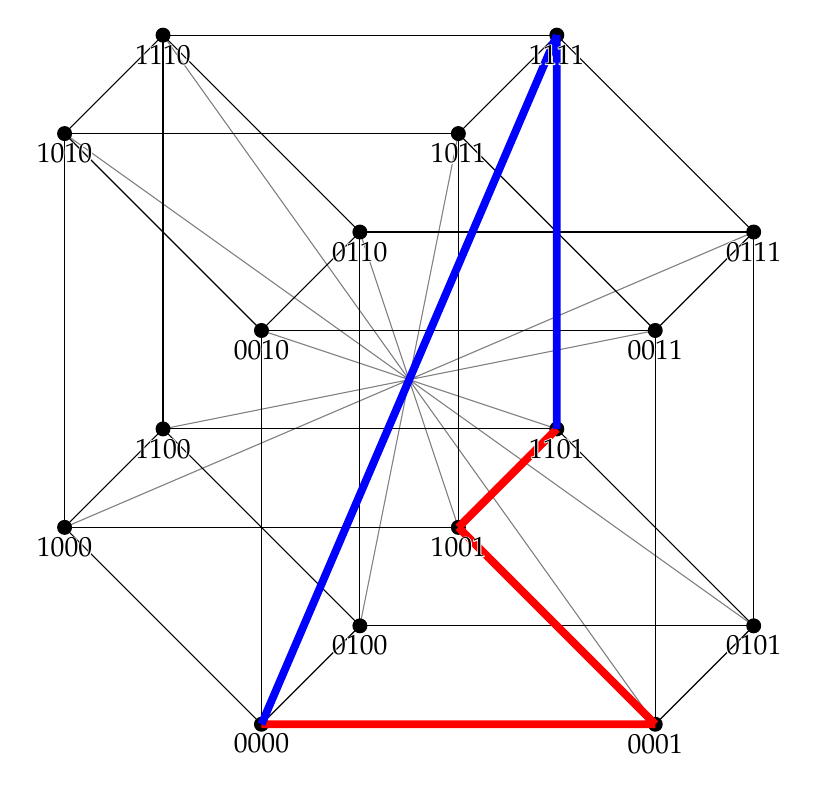
\begin{tikzpicture}[yscale=2.5, xscale=2.5, rotate=0]

\coordinate (0000) at (1,1);
\coordinate (0001) at (3,1);
\coordinate (0010) at (1,3);
\coordinate (0011) at (3,3);
\coordinate (0100) at (1.5,1.5);
\coordinate (0101) at (3.5,1.5);
\coordinate (0110) at (1.5,3.5);
\coordinate (0111) at (3.5,3.5);

\coordinate (1000) at (0,2);
\coordinate (1001) at (2,2);
\coordinate (1010) at (0,4);
\coordinate (1011) at (2,4);
\coordinate (1100) at (0.5,2.5);
\coordinate (1101) at (2.5,2.5);
\coordinate (1110) at (0.5,4.5);
\coordinate (1111) at (2.5,4.5);

\uncover<2->{
\draw[gray]
(0000) -- (1111)
(0010) -- (1101)
(0100) -- (1011)
(0110) -- (1001)
(1000) -- (0111)
(1010) -- (0101)
(1100) -- (0011)
(1110) -- (0001)
;
}

\draw
(0000) -- (0001)
(0010) -- (0011)
(0100) -- (0101)
(0110) -- (0111)
(1000) -- (1001)
(1010) -- (1011)
(1100) -- (1101)
(1110) -- (1111)
;


\draw
(0000) -- (0010)
(0001) -- (0011)
(0100) -- (0110)
(0101) -- (0111)
(1000) -- (1010)
(1001) -- (1011)
(1100) -- (1110)
(1101) -- (1111)
;

\draw
(0000) -- (0100)
(0001) -- (0101)
(0010) -- (0110)
(0011) -- (0111)
(1000) -- (1100)
(1001) -- (1101)
(1010) -- (1110)
(1011) -- (1111)
;

\draw
(0000) -- (1000)
(0001) -- (1001)
(0010) -- (1010)
(0011) -- (1011)
(0100) -- (1100)
(0101) -- (1101)
(0110) -- (1110)
(0111) -- (1111)
;




\filldraw[black] (0000)  circle (1pt);
\filldraw[black] (0001)  circle (1pt);
\filldraw[black] (0010)  circle (1pt);
\filldraw[black] (0011)  circle (1pt);
\filldraw[black] (0100)  circle (1pt);
\filldraw[black] (0101)  circle (1pt);
\filldraw[black] (0110)  circle (1pt);
\filldraw[black] (0111)  circle (1pt);

\filldraw[black] (1000)  circle (1pt);
\filldraw[black] (1001)  circle (1pt);
\filldraw[black] (1010)  circle (1pt);
\filldraw[black] (1011)  circle (1pt);
\filldraw[black] (1100)  circle (1pt);
\filldraw[black] (1101)  circle (1pt);
\filldraw[black] (1110)  circle (1pt);
\filldraw[black] (1111)  circle (1pt);


\uncover<3->{
	\draw[line width=1.0mm, red]
	(0000) -- (0001)
	(0001) -- (1001)
	(1001) -- (1101)
	;}

\uncover<4->{
	\draw[line width=1.0mm, blue]
	(0000) -- (1111)
	(1111) -- (1101)
	;}


\uncover<1->{

\draw (0000) node[below] {\contour{white}{0000}};
\draw (0001) node[below] {\contour{white}{0001}};
\draw (0010) node[below] {\contour{white}{0010}};
\draw (0011) node[below] {\contour{white}{0011}};
\draw (0100) node[below] {\contour{white}{0100}};
\draw (0101) node[below] {\contour{white}{0101}};
\draw (0110) node[below] {\contour{white}{0110}};
\draw (0111) node[below] {\contour{white}{0111}};

\draw (1000) node[below] {\contour{white}{1000}};
\draw (1001) node[below] {\contour{white}{1001}};
\draw (1010) node[below] {\contour{white}{1010}};
\draw (1011) node[below] {\contour{white}{1011}};
\draw (1100) node[below] {\contour{white}{1100}};
\draw (1101) node[below] {\contour{white}{1101}};
\draw (1110) node[below] {\contour{white}{1110}};
\draw (1111) node[below] {\contour{white}{1111}};
}




\end{tikzpicture}
\end{center}

\vspace{-5cm}
%\vspace{-10cm}
%\uncover<1-2>{\text{}\hspace{13cm}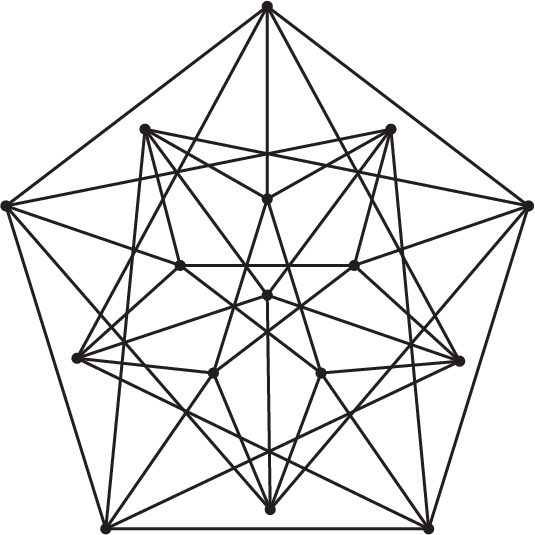
\includegraphics[scale=0.2]{clebsch3.png}}



\end{frame}






% \begin{frame}{Equivalent notions - 2 }{Subspace Arrangments}
%      For a set \(I \subset \cF\) let \(F_I \coloneqq \langle f \mid f \in I\rangle \). 
%     For \(t \in \bN\) consider the subspace arrangement \( \mathcal{A} \coloneqq \{F_I \mid dim(F_I) = t\}\). Then we have \(B_t(0) = \cup_{F_I \in \cA}F_I\). By exclusion/inclusion we have 
%     \begin{equation}
%         |B_t(0)| = \sum_{J \subset \cA} (-1)^{|J|+1}|\cap_{F \in J}F|
%     \end{equation}
%     An other version is obtained by considering the lattice: \(\cL_{\cA} \{\cap_{F \in J}F | J \subset \cA\}\) ordered by reverse inclusion.
%     \begin{equation}
%         |\bF^n_q \setminus B_t(0)|= \sum_{x \in \cL_{\cA}}\mu(\bF_q^n,x) card(x)
%     \end{equation}
%     Where \( \mu\) is the Möbius function of \(\cL_{\cA}\).

% \end{frame}

% \begin{frame}{Equivalent notions - 2 }{Subspace Arrangments}
% \begin{itemize}
% 	\item For some subspace arrangements the  Möbius function of some subspace arrangements is known.
% 	\item It may be useful to try to understand whether any of these can be induced by a projective metric. 
% 	\item This also points in the direction of trying to study the homology group of the lattice associated to a sphere of a projective metric.
% 	\item Ideas on how this might work are very welcome! :)
% \end{itemize}
% \end{frame}

% \begin{frame}{Equivalent notions - 3}{Known Hamming codes}
% 	A very important connection to Classical Coding theory is given by the following.
% 	\begin{definition}(Parent functions and Parent codes of $\cF$)
% 		The \myfont{parent functions} of $\cF$ are $\Ff_q$-linear functions $\varphi: \Ff_q^{\N} \to V$ such that $\langle \varphi( e_i ) \rangle = F_{\sigma(i)} \in \cF$ for some $\sigma(i) \in S_{\N}$.
% 		The \myfont{parent codes} of $\cF\subset \Gr_1(V)$ are the elements in the class $\bar \C := [\ker (\varphi)]$ where \([\ker (\varphi)]\) is the equivalence class of $\ker(\varphi)$ and \(\varphi\) is a parent function of $\cF$.
% 	\end{definition}

% Given \(v \in \cV\) the parent code \(\cC\) describes all the possible linear combinations of \(\cF\) that equal to \(v\).
% That is we have: \(v = \sum_{f \in \cF} a_ff = \sum_{f \in \cF} b_ff \) that is \(v = \varphi(a) = \varphi(b)\) if and only if \( a-b \in \cC\). 
% A series of important proprieties depends on this code, for example we have that:
% % \begin{observation}
% % \end{observation}
% If \(x \in \mathbb{F}_q^\mathbb{N}\) satisfies \(\wt_H(x) \leq \frac{d_H(\mathcal{C})}{2}\), then \(\wt_H(x) = \wt_\mathcal{F}(\varphi(x))\).


% \end{frame}








\begin{frame}{}{What can we do?}
\vspace{-1.5cm}
\uncover<2->{Singleton-type bound!\\~\\}

\uncover<3->{Let $V$ be an $n$-dim vector space over $\F_q$. Let $\cF$ be a spanning family for a projective metric.\\}
\uncover<4->{
\begin{definition*}
	\textnormal{
	Let $t \in \{0,1,2,\ldots,n\}$. We define $\mu_{\cF}(t)$ as the maximum cardinality of a subset $\cG \subseteq \cF$ satisfying
	\begin{enumerate}
		\item \uncover<5->{All $f_i \in \cG$ are linear independent from each other over $\F_q$;}
		\item \uncover<6->{All $v \in \langle \cG \rangle$ have $\wt_{\cF}(v) \leq t$.}
	\end{enumerate}
}
\end{definition*}
}

\uncover<7->{
\begin{theorem}[\textbf{General Singleton-type bound}] 

 \scalebox{1.1}{Let $\C \subseteq V$ be a subset and let $d = \min\{d_{\cF}(x,y) \,|\, x \neq y \in \C)\}$. Then}
	\[
	\scalebox{1.2}{$|\C| \leq q^{n - \mu_{\cF}(d-1)} \leq q^{n-d+1}$
}
	\]
\end{theorem}
}

\uncover<8->{
	\textbf{Coincides} with Singleton bounds for specific projective metrics!
}
\end{frame}

\begin{frame}{Characterization of projective metrics }{What can we do?}


Where two codes are equivalent if there exists a linear Hamming isometry sending one onto the other. The following result tells us that a projective metric is univocally determined by it's parent code.
\begin{theorem}
    
    Let $ \bar Pr_{\N}(V)$ be the set containing the equivalence classes of projective metrics on $V$ of size $\N$ and $\bar Gr_{\N-N}(\Ff_q^{\N})$ be the set containing the equivalence classes of subspaces of $\Ff^{\N}_q$ of dimension $\N - N$. Then there exists a bijection:
    \begin{align*}
    \Psi: \bar Pr_{\N}(V) &\to \bar Gr_{\N-N}(\Ff_q^{\N}) \\
    \bar w_{\cF} &\mapsto \bar \C_{\cF}
\end{align*}
    Where $\bar \C_{\cF}$ is the parent code of $\cF$.
\end{theorem}

\end{frame}
\begin{frame}{Characterization of projective isometries}{What can we do?}
    
\begin{definition}
    An \(\F\)-isometry is a linear isomorphism \(L:V \to V\) such that \(L(\cF) = \cF\). The set of \(\F\)-isometries, with the operation of composition, forms a group denoted as \(isom_{\F}(V)\).
\end{definition}

\begin{theorem}
Let \(stab_H(\C)\) be the stabilizer of the parent code \(\C\) respect to the Hamming isometries, then \(isom_{\cF}(V) \cong stab_H(\C)\)
\end{theorem}

% \begin{theorem}
%     \(isom_{\cF}(V) \cong stab_H(\C)\). The group isomorphism is given by \(\Psi: stab_H(\C) \to isom_{\cF}(V)\) where \(\Psi(F) = \hat F\), the unique \(\cF\)-isometry such that the following diagram commutes:
%     \[\begin{tikzcd}[ampersand replacement=\&]
%         V \arrow[r,"F"] \& V \\
%         \Ff_q^{\N} \arrow[u,"\varphi"] \arrow[r,"\hat F"'] \& \Ff_q^{\N} \arrow[u,"\varphi"']
%     \end{tikzcd}\]
% \end{theorem}
\end{frame}

% \begin{frame}{Constructions}{What can we do?}
% \vspace{-1cm}
% \uncover<2->

% \uncover<3->{
% We can define
% \[
% \wt_{\cF} \cup \wt_{\cG} := \wt_{\cF \cup \cG}
% \]
%  and
% \[
% \wt_{\cF} \otimes \wt_{\cG} := \wt_{\cF \otimes \cG}
% \]
% where $\cF \otimes \cG := \{\langle f_i \rangle \otimes \langle g_i \rangle \,\,|\,\, \langle f_i \rangle \in \cF, \,\langle g_i \rangle \in \cG \}$\\~\\
% }

% \uncover<4->{
% \textbf{Example}\\

% Let $\cF = \{\text{all 1-dim subspaces of } V\}$. Then $\wt_{\cF}(x) = 1$ for all $x\neq 0$. This is the \textbf{discrete weight} $\wt_{\operatorname{Dis}}$.\\~\\
% }

% \uncover<5->{

% \textbf{Examples}\\
% \begin{itemize}
% 	\item \uncover<6->{
% 		\scalebox{1.2}{$\wt_{\operatorname{Dis}} \otimes \wt_{\operatorname{Dis}} = \wt_{\operatorname{Rank}}$} \\}%\,\,\,\, (on $V_1 \otimes V_2$)
% 	\item \uncover<7->{\scalebox{1.2}{$\wt_{\operatorname{H}} \otimes \wt_{\operatorname{Rank}} = \wt_{\operatorname{Sum-rank}}$}\\}
% 	\item\uncover<8->{ \scalebox{1.2}{$\wt_{\operatorname{Dis}} \otimes \wt_{\operatorname{H}} = \wt_{\operatorname{Row}}$}\\}
% 	\item \uncover<9->{\scalebox{1.2}{$\wt_{\operatorname{H}} \otimes \wt_{\operatorname{Dis}} = \wt_{\operatorname{Column}}$}\\}
% 	\item \uncover<10->{\scalebox{1.2}{$\wt_{\operatorname{Row}} \cup \wt_{\operatorname{Column}} = \wt_{\operatorname{Cover}}$}}
% \end{itemize}

% }
% \end{frame}


\begin{frame}
    Equivalent notions of \(\wt_{\mathcal{F}}(\cdot)\) in different contexts:\\
    
    \begin{itemize}
        \item \uncover<2->{\textbf{Graph theory:}\\
            Cayley graph of \(\mathbb{F}_q^n\) with generating set \(\mathcal{F}\); $\wt_{\mathcal{F}}(v)$ is the graph distance between \(v\) and \(0\).\\}
        
        \uncover<4->{\item \textbf{Coding theory:}\\
            Certain code \(\mathcal{C}\) (depends on \(\mathcal{F}\)); $\wt_{\mathcal{F}}(v)$ is the Hamming weight of the coset \(v+\mathcal{C}\).\\}
        
        \uncover<6->{\item \textbf{Projective geometry:}\\
            Flats spanned by points in \(\mathcal{F}\); $\wt_{\mathcal{F}}(v)$ is the smallest rank of such a flat that contains \(v\).\\}
            And \(\wt_\mathcal{F}\)-isometries are simply homographies fixing \(\mathcal{F}\).
        \item \uncover<8->{\textbf{Subspace arrangments:} \\
			A ball of size \(t\) in projective metric corresponds to the size of the \textbf{subspace arrangement} generated by subsets of \(\cF\) of size less than \(t\).     
			}
		\item \uncover<10->{\textbf{Matroid theory:}} \\ \uncover<11->{We can see the Matroid Associated to the family \(\cF\). This seem do describe well the first two layers of the intersection lattice.}
			
        \uncover<12->{\item \textbf{Q:} General ways to calculate \(\wt_{\mathcal{F}}(v)\)?\\}
        \uncover<13->{\textbf{Q:} For fixed \(t\), how many \(v\) have \(\wt_{\mathcal{F}}(v) = t\)? \(\rightarrow\) Hamming-like bound.}
        
        \uncover<14->{\item Please let me know if you know a (partial) answer in any of these contexts!}
    \end{itemize}
\end{frame}


\begin{frame}{}{Current research}
\vspace{-0.5cm}
\begin{itemize}
\item Algorithms for calculating  $\wt_{\cF}(v)$ for $v \in V$
\item Are there general methods for obtaining sphere sizes $|\{v \in V \,|\, \wt_{\cF}(v)=t\}|$ for $t \in \mathbb{N}$?
\item Is there a natural way do generilize other concepts of coding theory? Dual Codes? Perfect Codes? ecc...
\item Approach?: using poset lattice of projective metrics, where $\wt_{\cF} \preccurlyeq \wt_{\cG} $ iff $\cF \subseteq \cG $
\end{itemize}


\begin{center}
	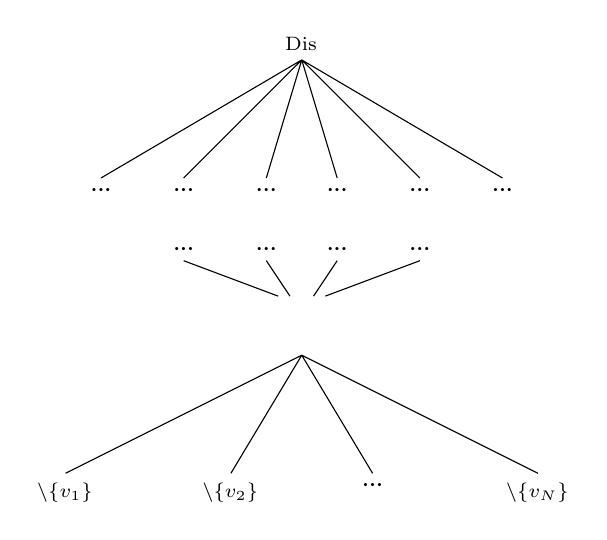
\begin{tikzpicture}[yscale=1.5, xscale=1.5, rotate=0]
	
	\draw (0,0) node[above] {$\wt_{\operatorname{Dis}}$}--(-1, -1) node[below] {...}
	(0,0) --(-0.3, -1) node[below] {...}
	(0,0) --(0.3, -1) node[below] {...}
	(0,0) --(1, -1) node[below] {...}
	(0,0) --(1.7, -1) node[below] {...}
	(0,0) --(-1.7, -1) node[below] {...}
	;
	
	
	\draw (0,-2.5) node[above] {$\wt_{\cF}$}--(-2, -3.5) node[below] {$\wt_{\cF \setminus \{v_1\}}$}
	(0,-2.5) --(-0.6, -3.5) node[below] {$\wt_{\cF \setminus \{v_2\}}$}
	(0,-2.5) --(0.6, -3.5) node[below] {...}
	(0,-2.5) --(2, -3.5) node[below] {$\wt_{\cF \setminus \{v_N\}}$}
	;
	
	\draw (-0.2,-2) -- (-1, -1.7) node[above] {...}
	(-0.1,-2) -- (-0.3, -1.7)  node[above] {...}
	(0.1,-2) -- (0.3, -1.7)  node[above] {...}
	(0.2,-2) -- (1, -1.7)  node[above] {...}
	;
	
\end{tikzpicture}
\end{center}



\end{frame}




\end{document}